\section{Radiation-Tolerant Design}
\label{rt_design}
The goal of radiation-tolerant design is to limit the potential damage caused by radiation effects as described in section \ref{rad_effect_cmos}. Some of these effects can only be limited by a careful layout of the die or by the intrinsic properties of the chosen CMOS technology. However, SEUs can be reduced and mitigated by a combination of digital design. The methods for radiation hardening are usually dependent on redundancy either in space or in time. 

A common method is the use of triple module redundancy (TMR). In this method, each memory element (i.e. register) and the corresponding combinatorial logic are instantiated three times. The outputs from these three registers are then passed to a voting system, which outputs the majority vote. The voting system itself is also triplicated to minimize the chance of a SET upset. If a single voter is used and is sampled during the SET, an error will occur in the system, thus leading to a single-point of failure. To avoid the build-up of errors in the 3 different paths, the feedback loop of a state machine should be taken from the voted result. An example of a TMR radiation hardening can be seen in figure \ref{fig:spatial_triplication}.

\begin{figure}[H]
    \centering
    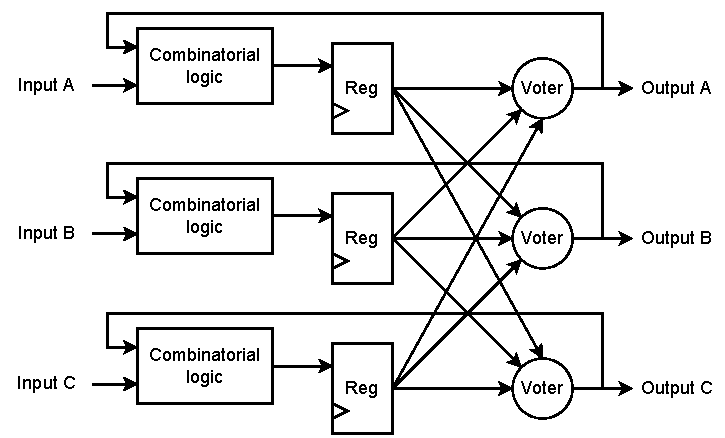
\includegraphics[width=0.7\linewidth]{subfiles/imgs/spacialTriplication.drawio (1).pdf}
    \caption{Shows a spatial radiation hardening technique using triple module redundancy.}
    \label{fig:spatial_triplication}
\end{figure}

This added redundancy would lose many of its radiation hardness benefits if the triplicated registers are placed close together on the chip die as this would increase the chance of an SEU happening on multiple registers from the same charged particle. Therefore the placement of these registers is restricted in the physical layout such that a minimum distance is enforced. 
%To reduce the chance of multiple errors from the same charged particle to a few percent, the distance has to be at least \SI{15}{\um} for \SI{65}{nm} technology \todo{kilde}. 
From this, it is clear that TMR increases radiation hardness by using space and power consumption (increased due to increase in hardware) as a trade-off. This increase in power and area is not cheap as the heat generated needs to be transported away from the detector and the space itself is limited inside the detector. Therefore to limit the disadvantages, the TMR is usually only done to the control path of a state machine. This is done as errors in the data path are limited in time, while an error in the control path can result in complete failure of the chip. At CERN, a tool has been developed for this method of radiation hardening named TMRG.

Another way of radiation hardening is the use of temporal spacing and is done by delaying the clock signal. The registers between combinatorial logic are triplicated, while the combinatorial logic itself, is not. Instead, the clock signal for each of the three registers is delayed, such that the SEU has a high statistical probability of having passed. This results in the SEU only affecting one register. It is then possible to use the same voting system as in TMR to achieve a corrected output. An example of this can be seen in figure \ref{fig:spatial_triplication}.

\begin{figure}[H]
    \centering
    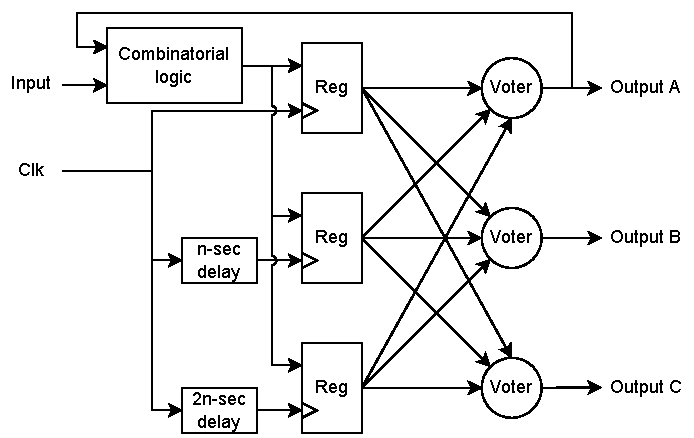
\includegraphics[width=0.7\linewidth]{subfiles/imgs/temporalTriplication.drawio.pdf}
    \caption{Shows a temporal radiation hardening technique where clock signals are delayed.}
    \label{fig:temporal_triplication}
\end{figure}

This method does not have the same minimum distance requirement as the TMR hardening technique as the registers sample at different timestamps. Instead, there is a temporal spacing requirement. 
%To lower the chance of affecting multiple registers to an acceptable level, the temporal spacing has been found to be at least \SI{200}{ps} \todo{kilde}. 
This method does not require a triplication of the  combinatorial logic and therefore saves on space and power consumption. However, it does make the timing analysis and closure difficult and this only gets more problematic as the frequency increases. 

Even though temporal radiation hardening has multiple advantages in the form of space and power consumption, the TMR is chosen due to its simpler implementation. This is due to the problematic nature of timing closure for the temporal radiation hardening, but also due to the existence of an already-developed tool for performing TMR. 

